\documentclass{article}
\title{P5 Report}
\author{Nick Werle}
\usepackage{hyperref}
\usepackage{graphicx}
\makeatletter
\def\maxwidth#1{\ifdim\Gin@nat@width>#1 #1\else\Gin@nat@width\fi}
\makeatother

\begin{document}
\maketitle
\section{Preamble}
Files will be submitted per instructions to pilot, and all work will be available on github at: \url{https://github.com/NickWer/CEG3900_P5} in two days.

\section{Task 1}
Deliverables: See devDocs.pdf and userDocs.pdf in the Task1 folder on github, see images 1-4 for screenshots.

Status report: I believe my user docs are sufficient for this game. I believe my dev docs, while they are not super in depth, provide an adequate high level view of the application's classes. They do not address specific implementation details however.

Experience: The user docs were not bad. The game is kind of fun but the difficulty is low and then becomes somewhat impractically difficult after a certain point. Very hard to play while the phone is plugged in. The dev docs were kind of a pain, but realistically it's not too terrible to understand all the source code.

	\begin{figure}[ht]
		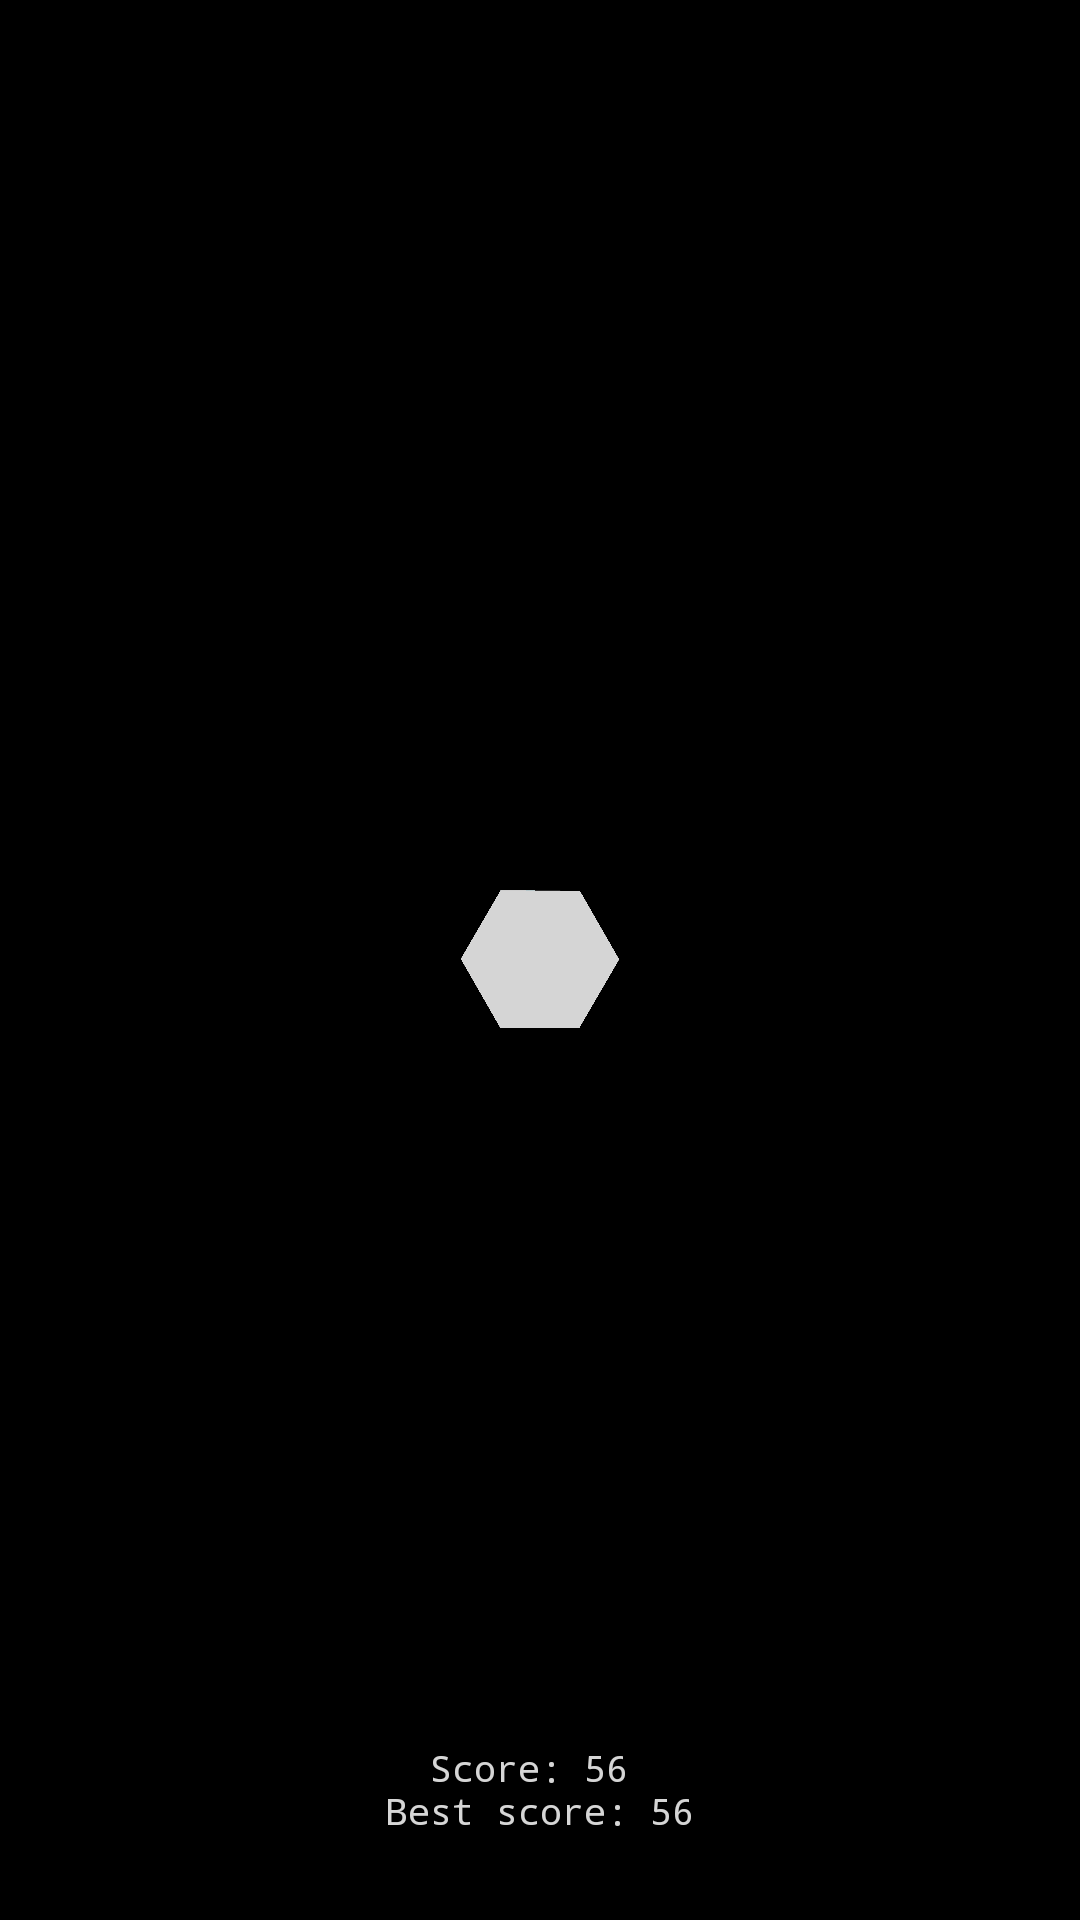
\includegraphics[width=3in]{img/t1s1.png}
		\centering
		\caption{Task 1 - Starting screen}
	\end{figure}
	\begin{figure}[ht]
		
\includegraphics[width=3in]{img/t1s2.png}
		\centering
		\caption{Task 1 - A game has begun - the center hexagon is much smaller}
	\end{figure}
	\begin{figure}[ht]
		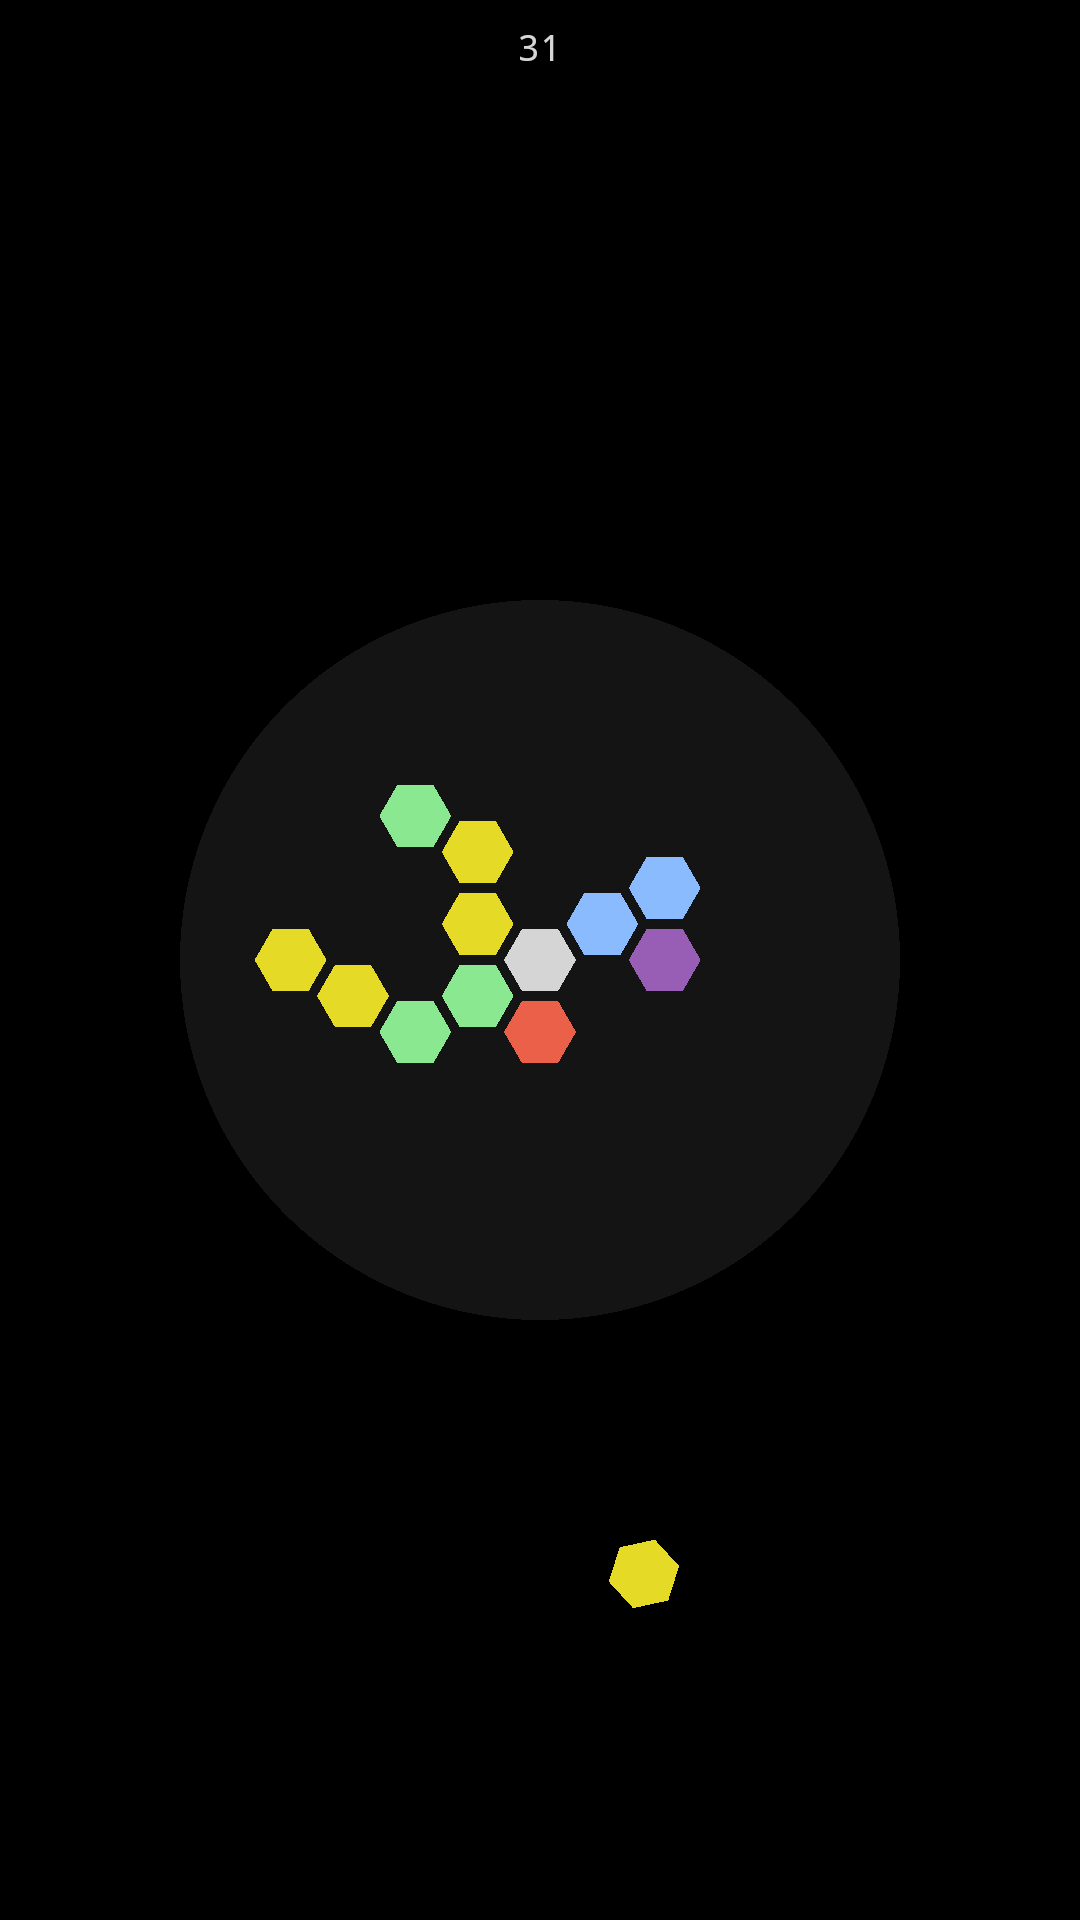
\includegraphics[width=3in]{img/t1s3.png}
		\centering
		\caption{Task 1 - Part 1 of 2 - Demonstrating how a chain can remove more than just 3 blocks}
	\end{figure}
	\begin{figure}[ht]
		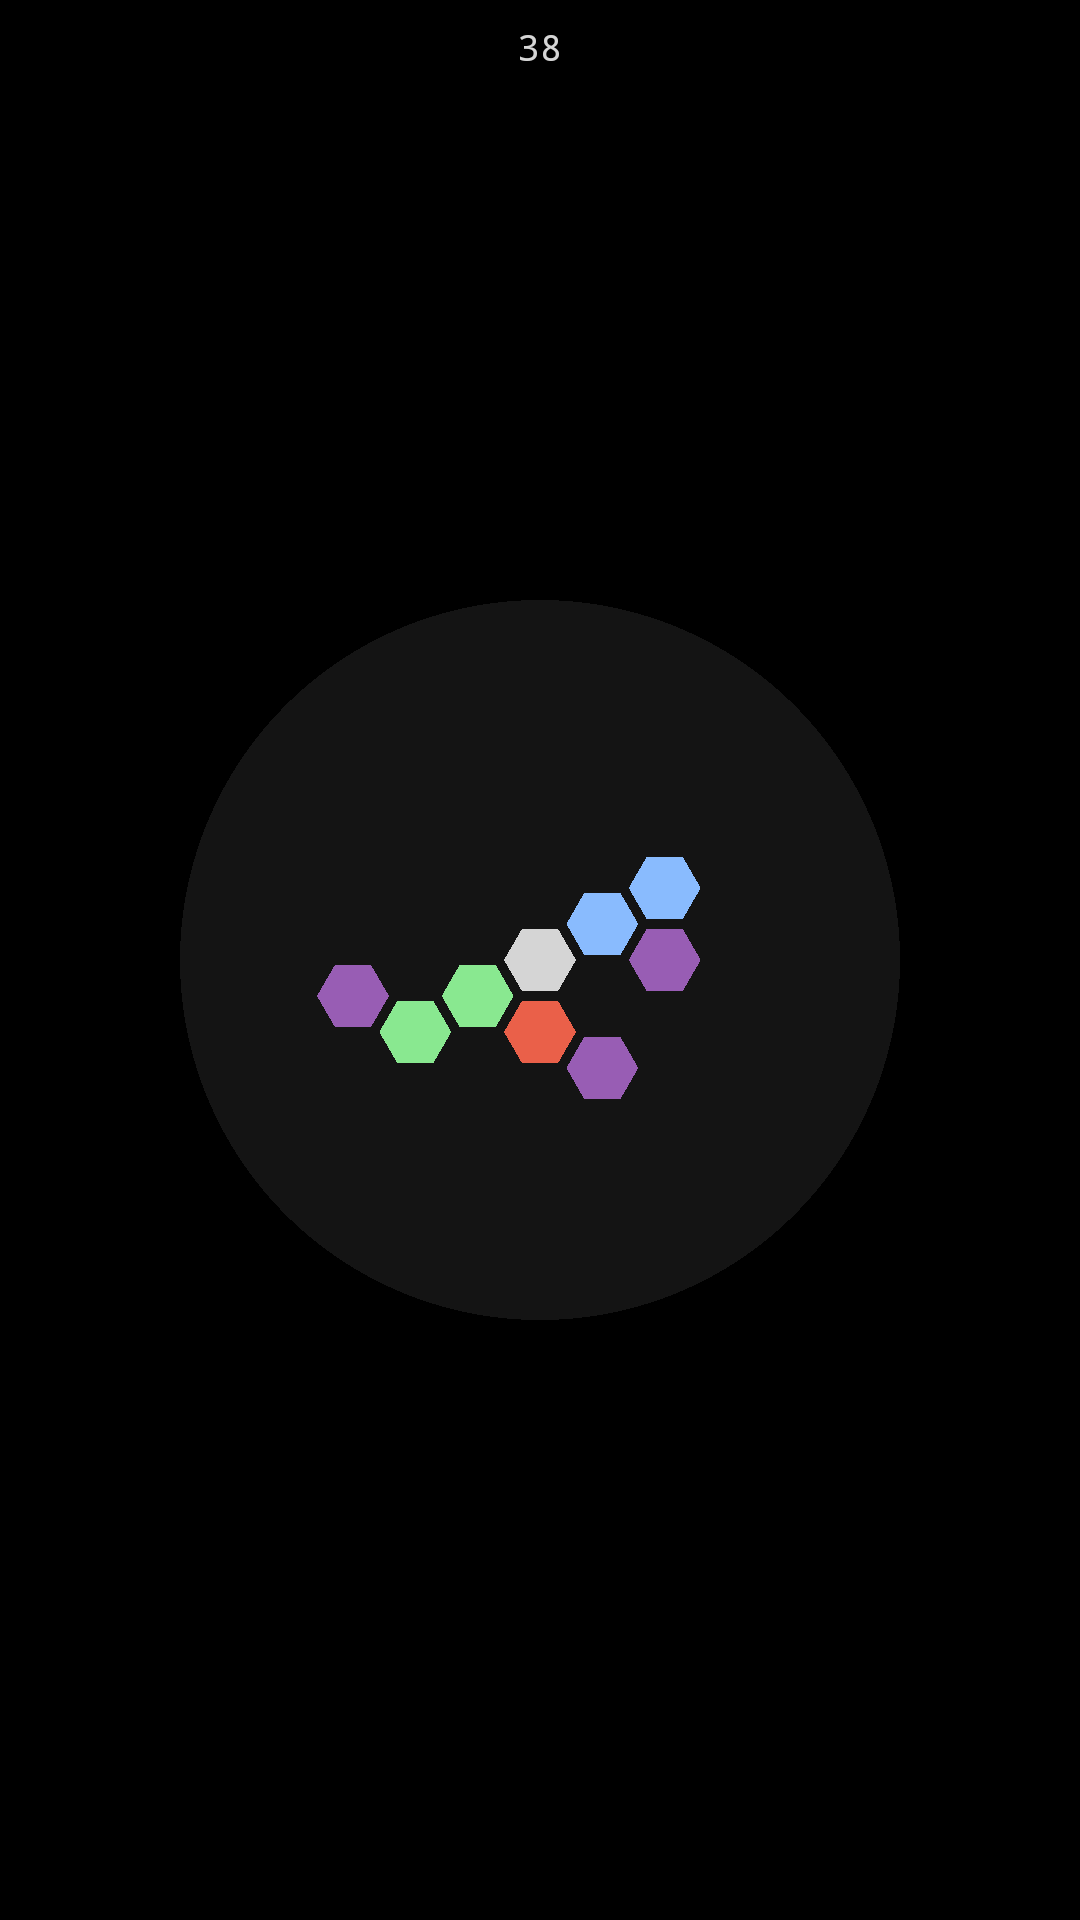
\includegraphics[width=3in]{img/t1s4.png}
		\centering
		\caption{Task 1 - Part 2 of 2 - Demonstrating how a chain can remove more than just 3 blocks}
	\end{figure}

\clearpage
\section{Task 2}
Deliverables: See screenshots 5-8. My MS Azure account is linked to my wright state email address, werle.3@wright.edu

Status Report: The application works as expected. Uploads and recalls images without hiccup.

Experience Report: Building the APK was very easy. Honestly registering to MS Azure was harder, because of a glitch with wright state's single sign on. I had to go incognito to get it to work. Other than that, and trying to find my account key, it was not a terrible experience. A promising platform, for sure, with a generous trial offer.

	\begin{figure}[ht]
		
\includegraphics[width=3in]{img/t2s1.png}
		\centering
		\caption{Task 2 - Starting screen}
	\end{figure}
	\begin{figure}[ht]
		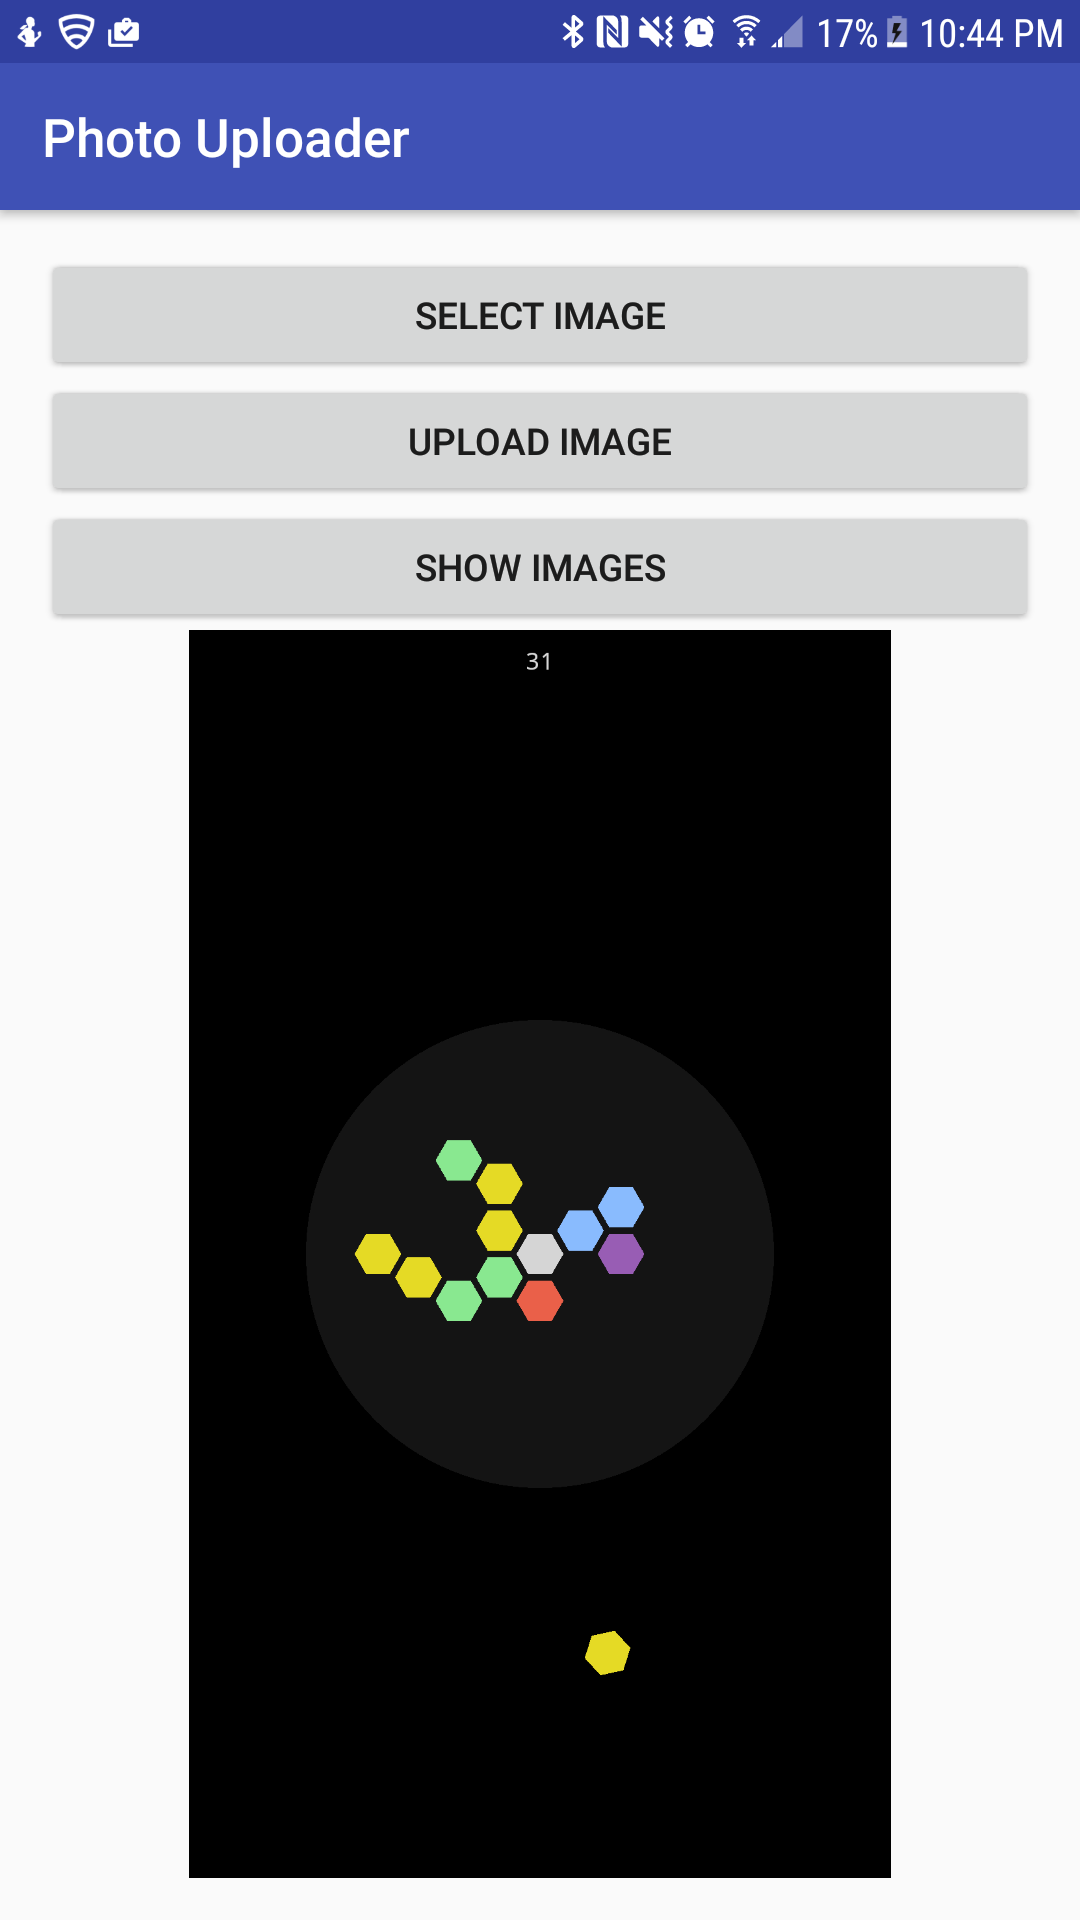
\includegraphics[width=3in]{img/t2s2.png}
		\centering
        \caption{Task 2 - An image about to be uploaded}
	\end{figure}
	\begin{figure}[ht]
		
\includegraphics[width=3in]{img/t2s3.png}
		\centering
        \caption{Task 2 - List of images that have been uploaded}
	\end{figure}
	\begin{figure}[ht]
		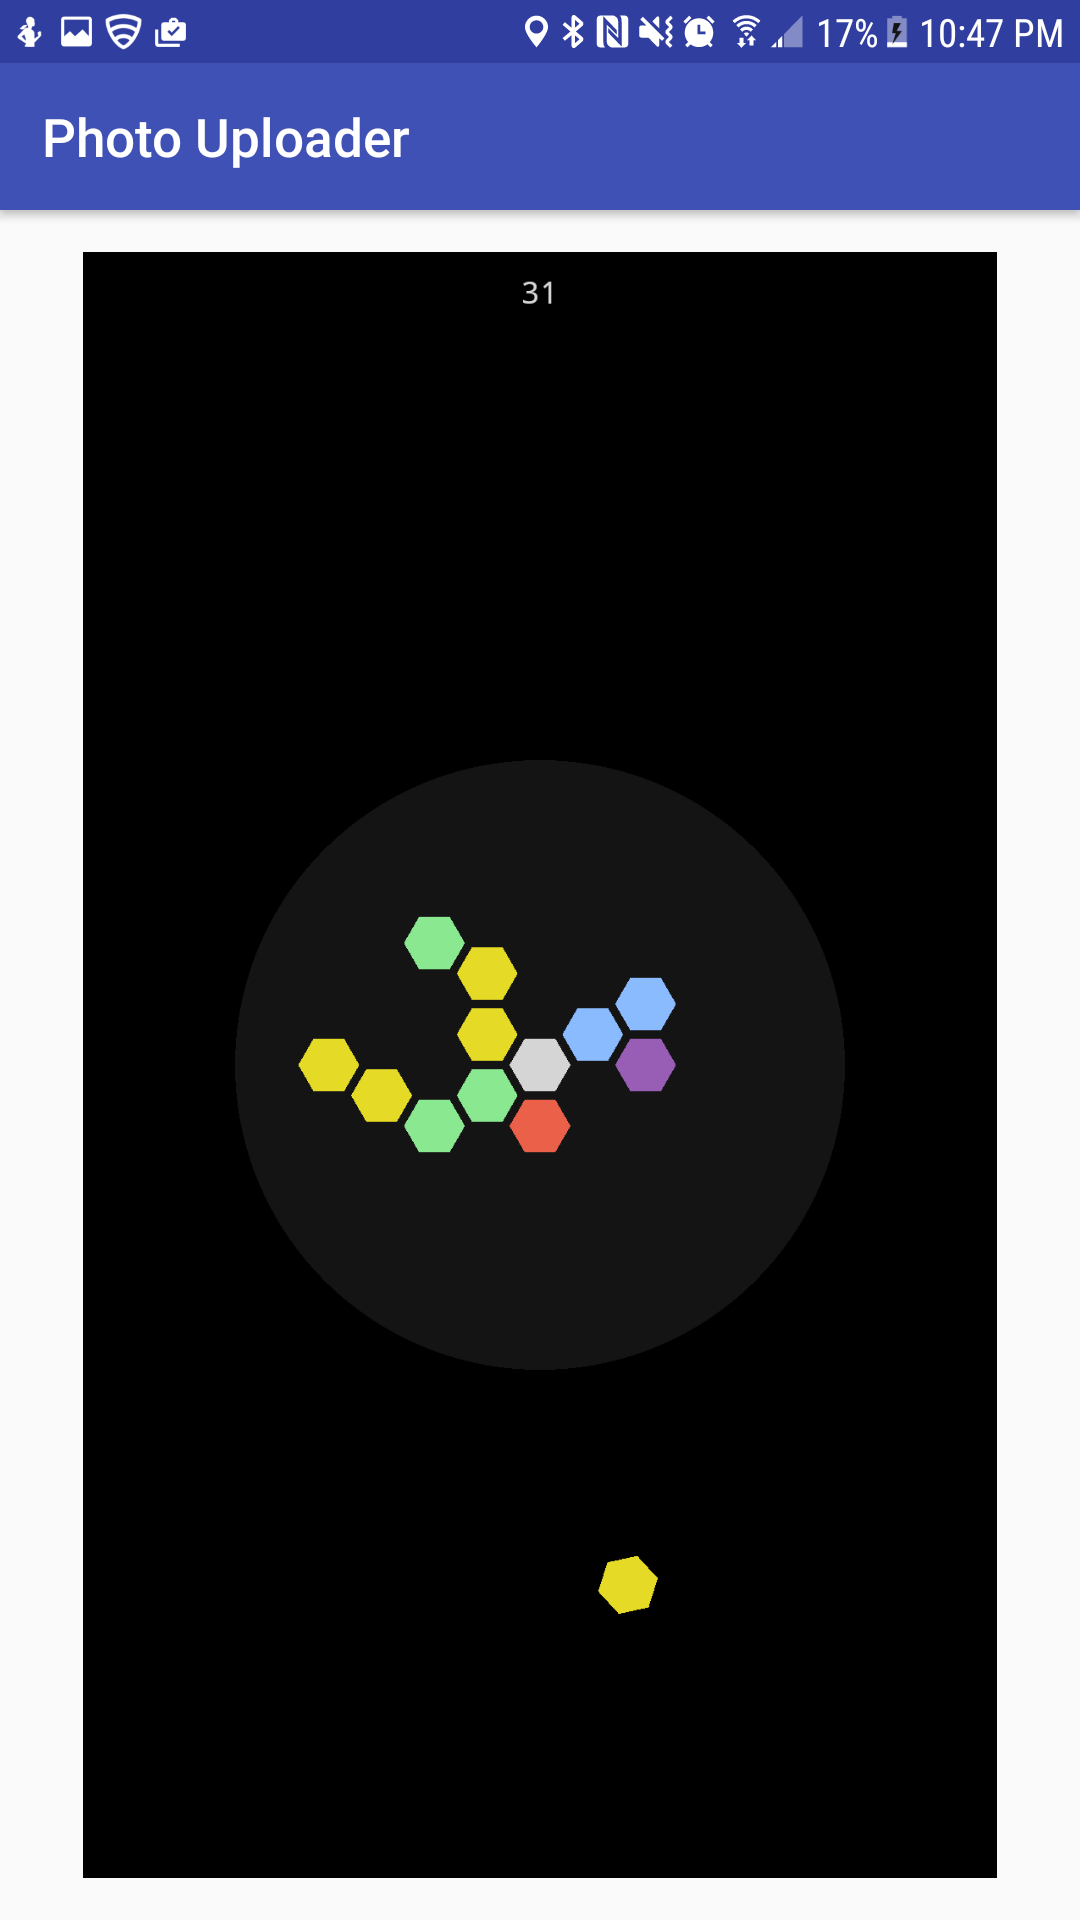
\includegraphics[width=3in]{img/t2s4.png}
		\centering
		\caption{Task 2 - The uploaded image}
	\end{figure}


\clearpage
\section{Task 3}
Deliverables: See screenshots 9-12. Google cloud platform account is linked to my private throwaway gmail address.

Status Report: It mostly works. I tried running one of the later parts of the tutorial that allows users to upload images and it didn't like it, but I honestly spent literally 2-3 hours on this task because of some misleading information regarding setting up the authentication credentials needed for the google cloud SDK. So basically, I'm just trilled that it works at all - and in fact, it works perfectly fine for everything that I tested \textit{except} image uploads.

Experience report: As I just mentioned, this one was particularly challenging for me.
Took a decent bit to get the environment set up correctly, and then I was recieving a mysterious 401 error that would cause my application to crash before it had even started.
I had honestly written up a several page, with screenshot explanation of the situation that I was going to submit instead, when I found the solution.
The issue was that you need to set up credentials for the application, but when you go to do so, it says you don't need any credentials and that the default will work just fine.
What was not clear was that you had to do something to enable those default credentails (which doesn't seem very default to me...).
Anyways, it works now, which is what matters I suppose.


	\begin{figure}[ht]
		
\includegraphics[width=\maxwidth{5in}]{img/t3s1.png}
		\centering
		\caption{Task 3 - The initial screen}
	\end{figure}
	\begin{figure}[ht]
		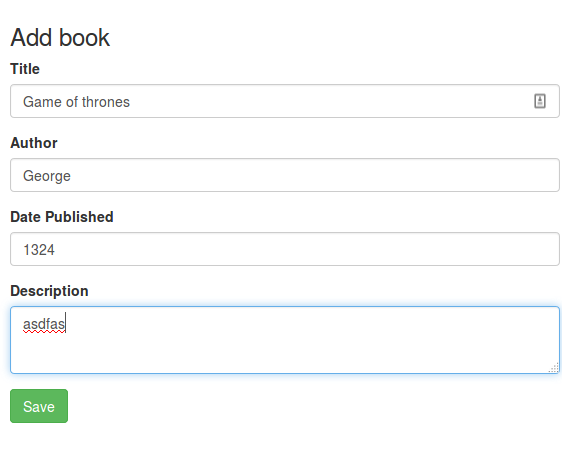
\includegraphics[width=\maxwidth{5in}]{img/t3s2.png}
		\centering
        \caption{Task 3 - Creating a book}
	\end{figure}
	\begin{figure}[ht]
		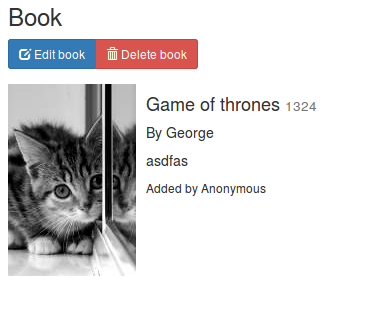
\includegraphics[width=\maxwidth{5in}]{img/t3s3.png}
		\centering
        \caption{Task 3 - The book I created}
	\end{figure}
	\begin{figure}[ht]
		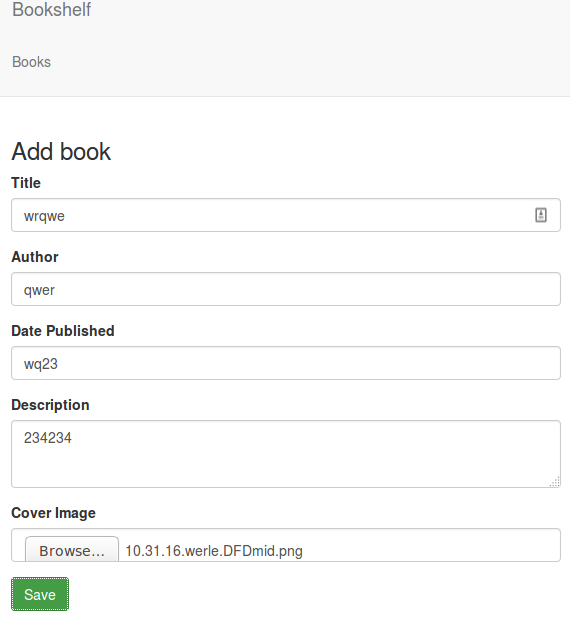
\includegraphics[width=\maxwidth{5in}]{img/t3s4.png}
		\centering
		\caption{Task 3 - The image upload portion. Almost works, but there's an exception when I hit submit that lacks an obvious solution, given that the tutorial seems to think it should just work out of the box.}
	\end{figure}
	
\clearpage
\section{Task 4}
Deliverables: See screenshots 13-16

Status Report: My tagging system works and updates live using firebase. The rendering is a bit janky but I think it is sufficient given the scope of the assignment. Really it's nothing fancy but it works more or less as I would expect

Experience Report: I didn't think this one was too bad, although at one point I tried to integrate java 8 and it was kind of a disaster because a bunch of compatibility issues arose, and it ended up just being easier to write the for loops. Honestly I found firebase to be extremely easy to integrate into the application. It's very intuitive.

	\begin{figure}[ht]
		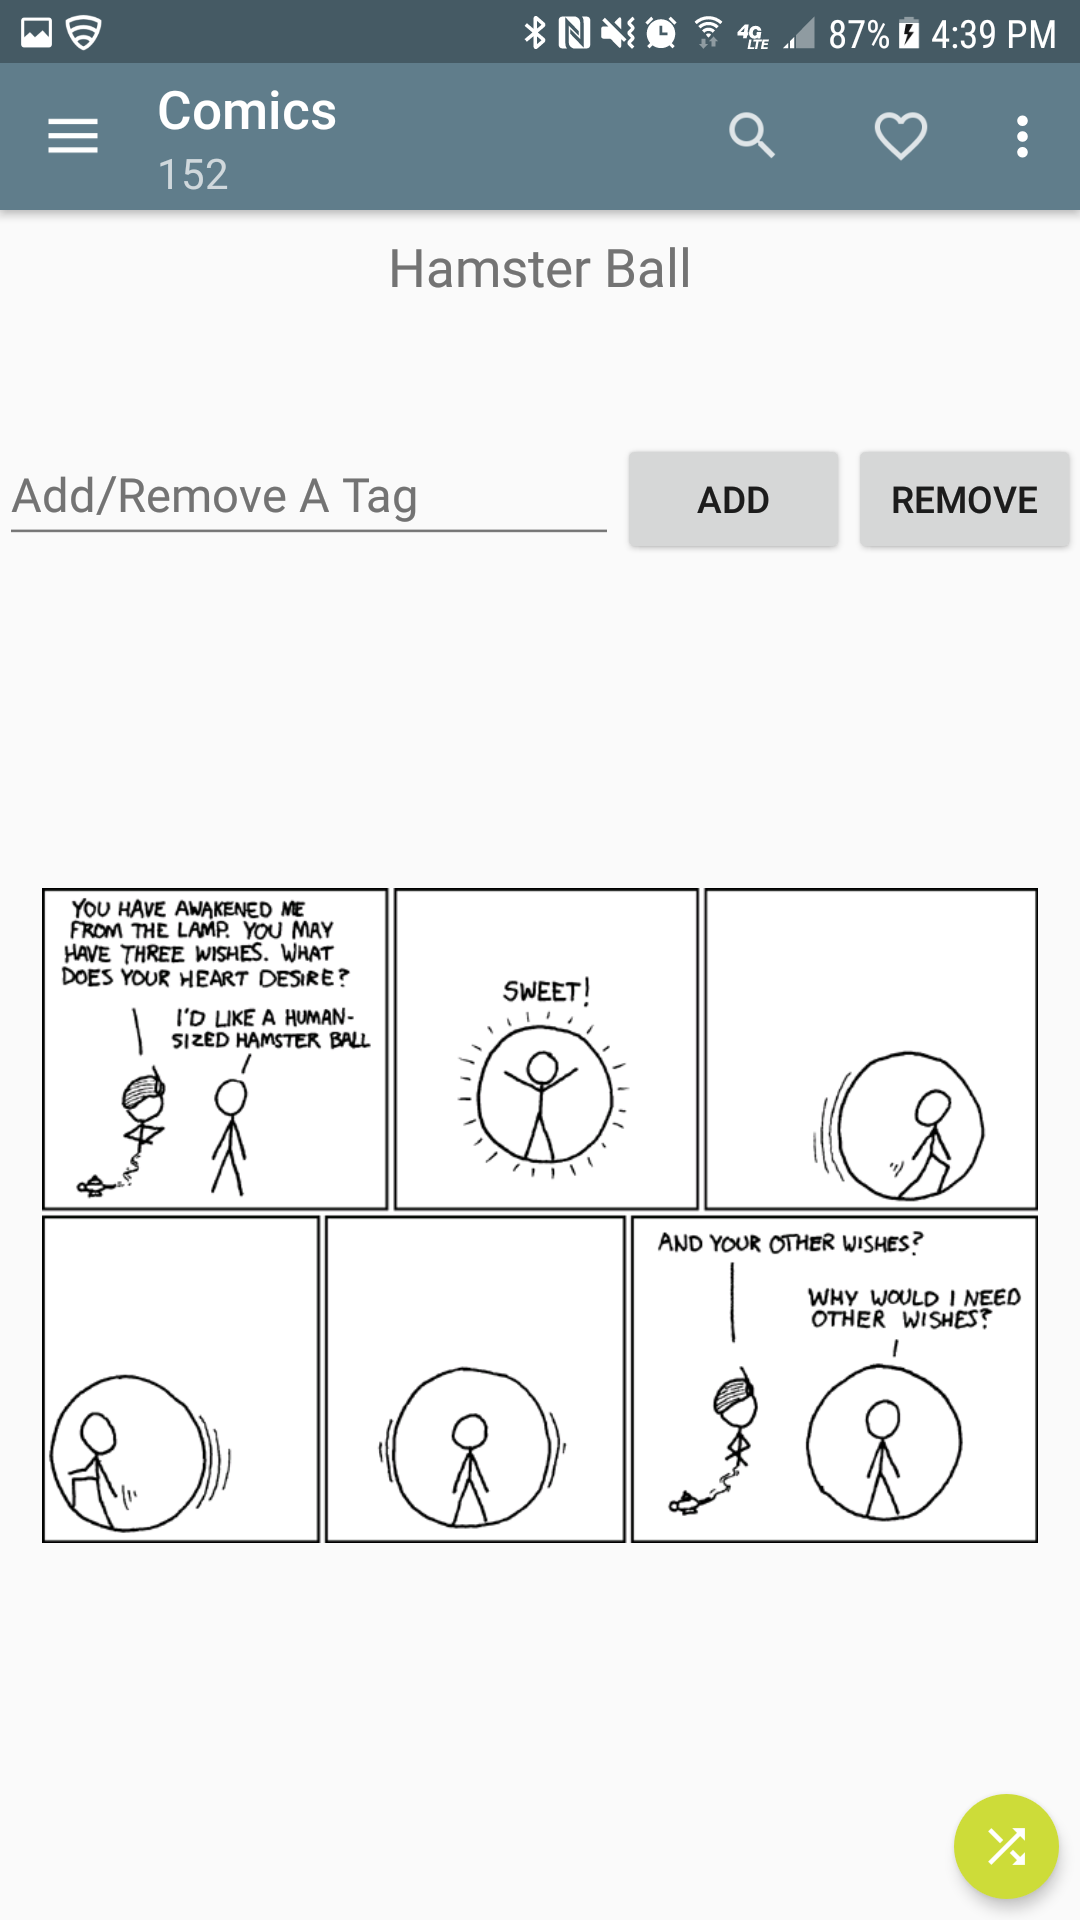
\includegraphics[width=\maxwidth{3in}]{img/t4s1.png}
		\centering
		\caption{Task 4 - A random comic with no tags}
	\end{figure}
	\begin{figure}[ht]
		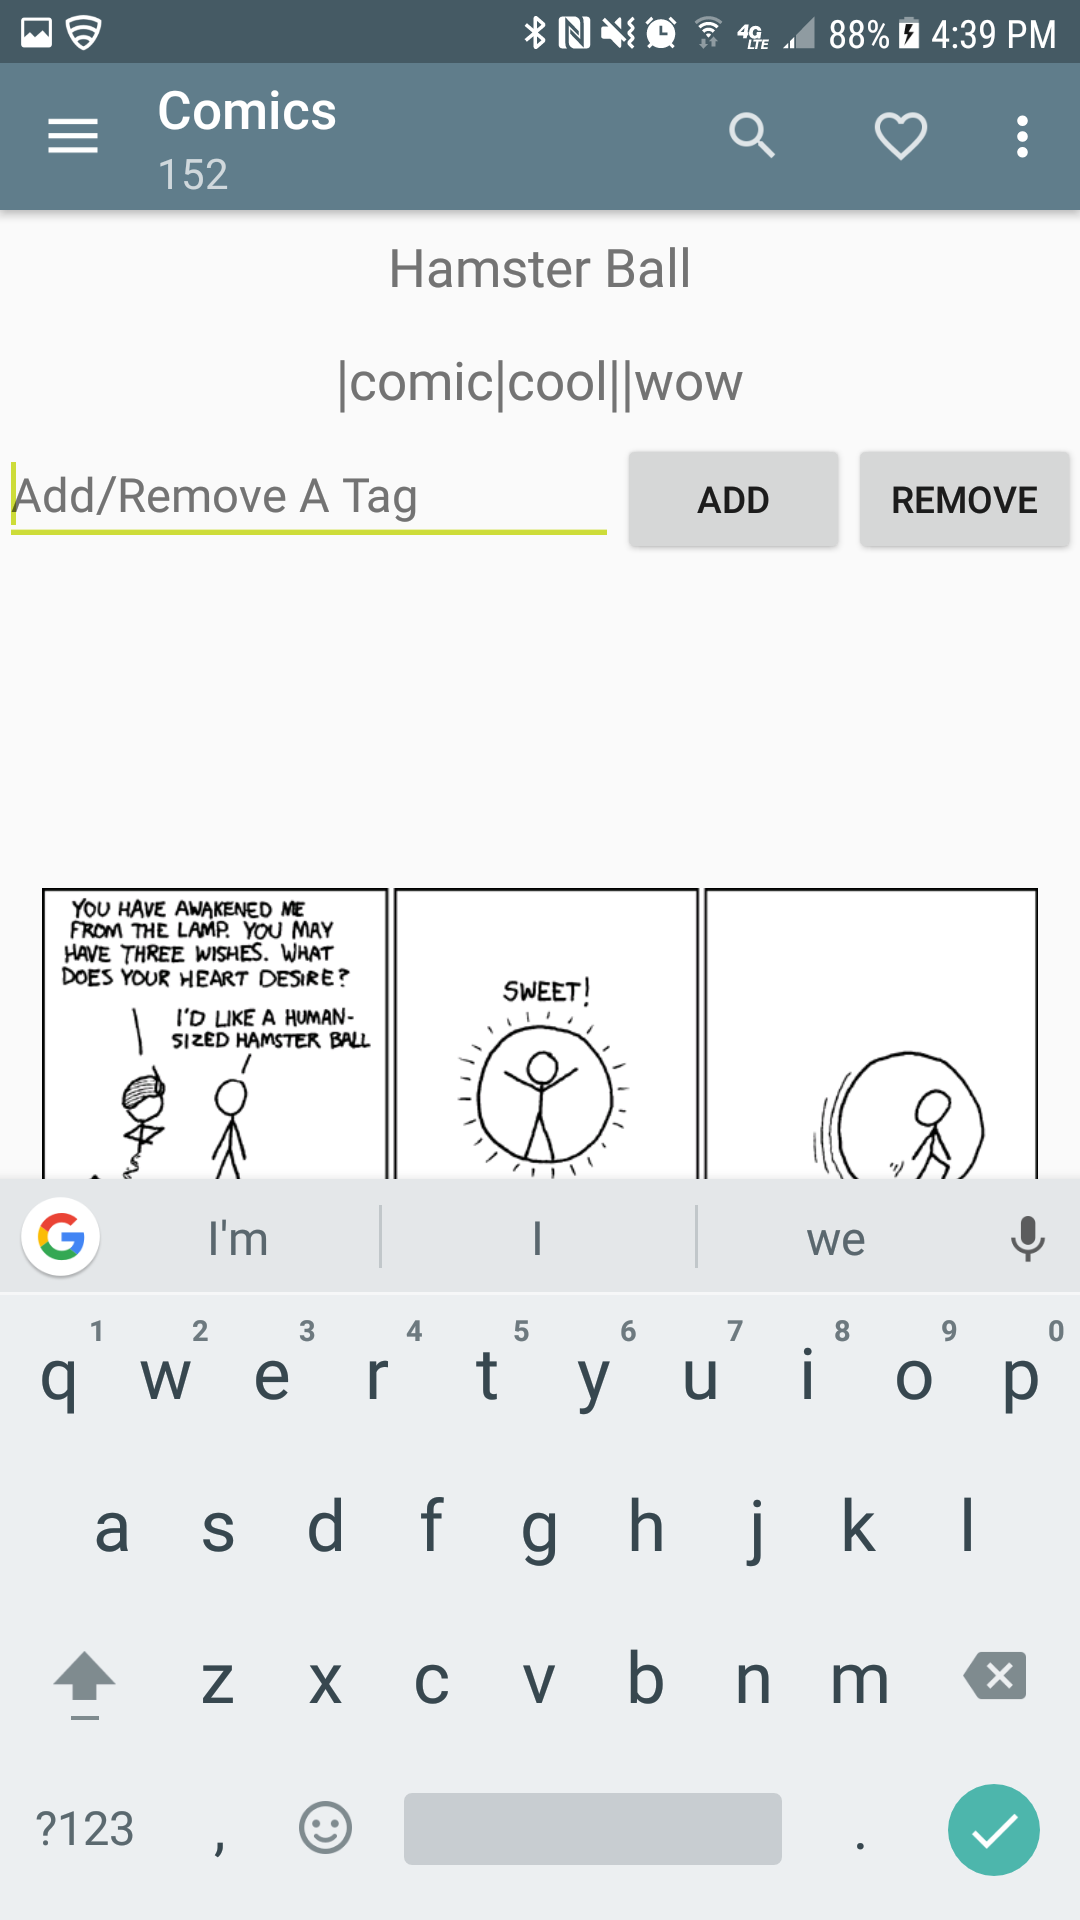
\includegraphics[width=\maxwidth{3in}]{img/t4s2.png}
		\centering
        \caption{Task 4 - The comic but with three tags}
	\end{figure}
	\begin{figure}[ht]
		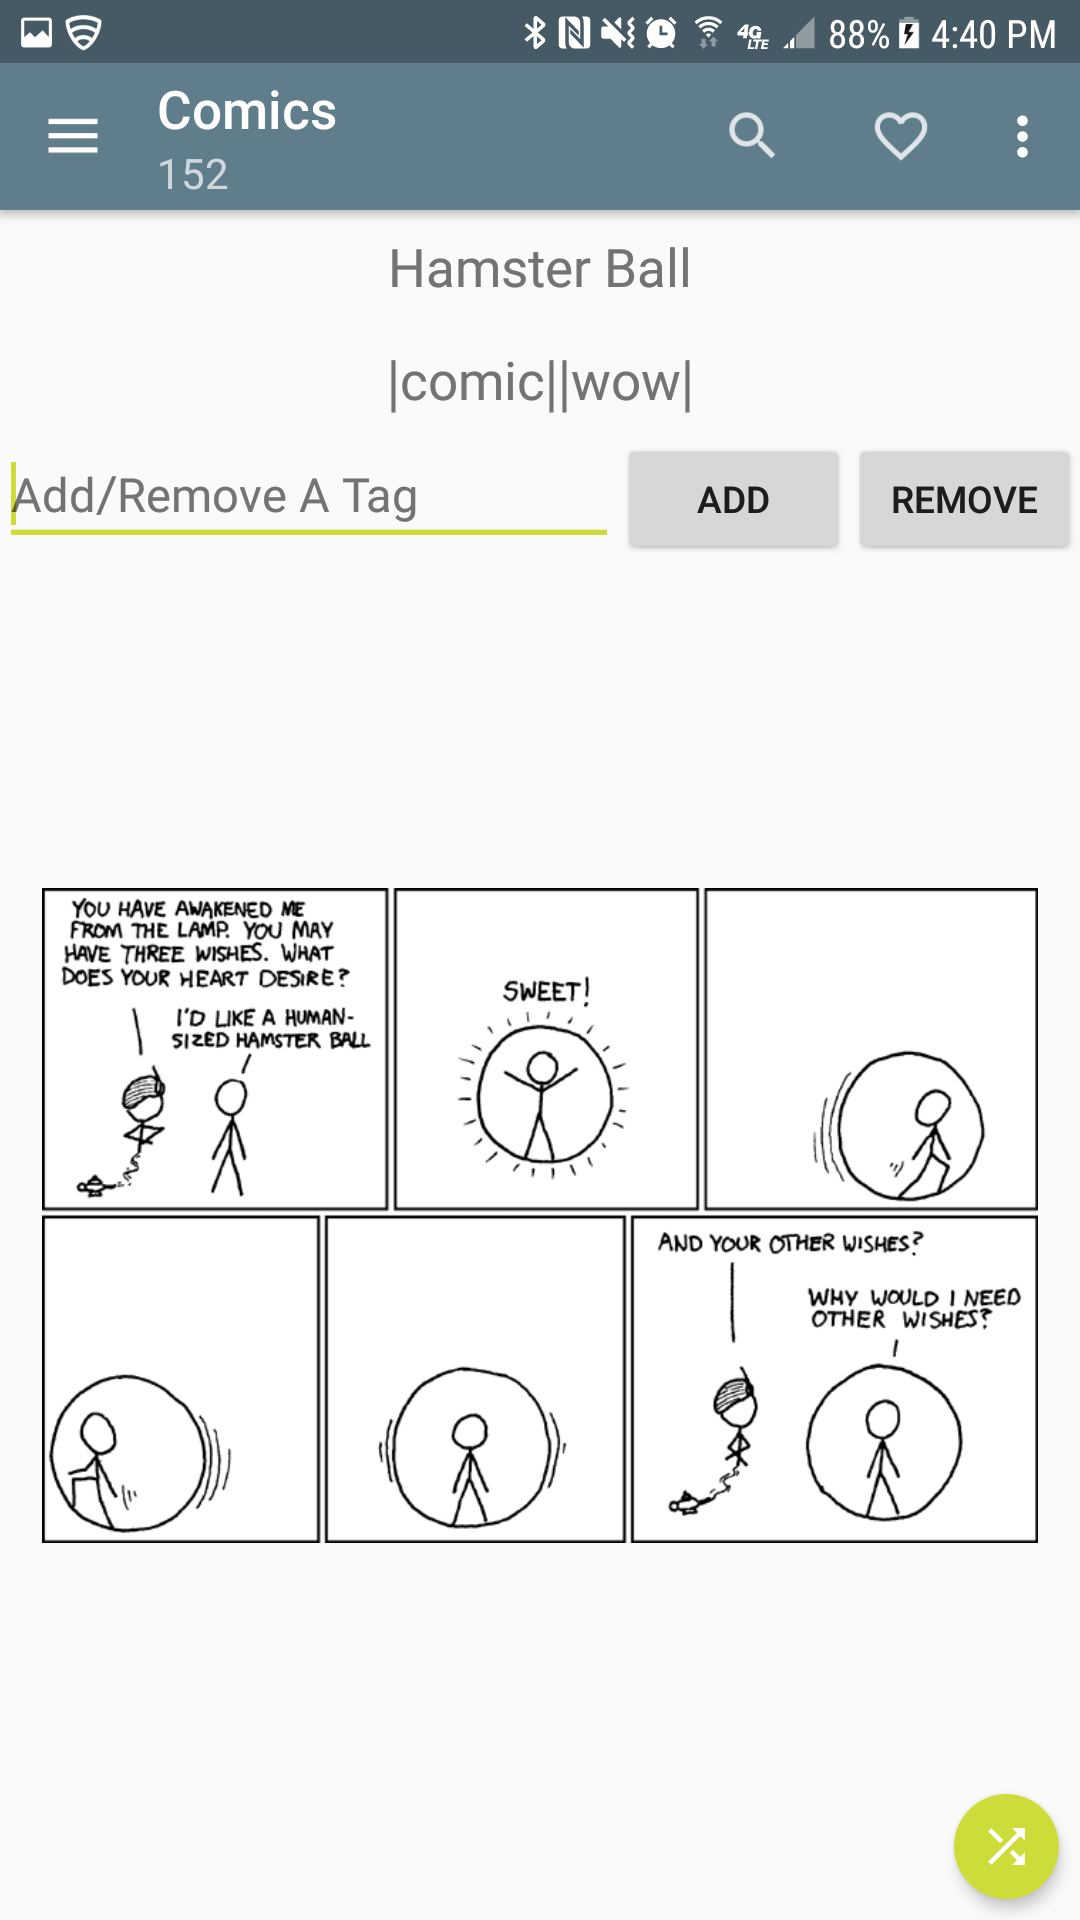
\includegraphics[width=\maxwidth{3in}]{img/t4s3.png}
		\centering
        \caption{Task 4 - Removed the tag "cool" by typing "cool" into the box and hitting remove}
	\end{figure}
	\begin{figure}[ht]
		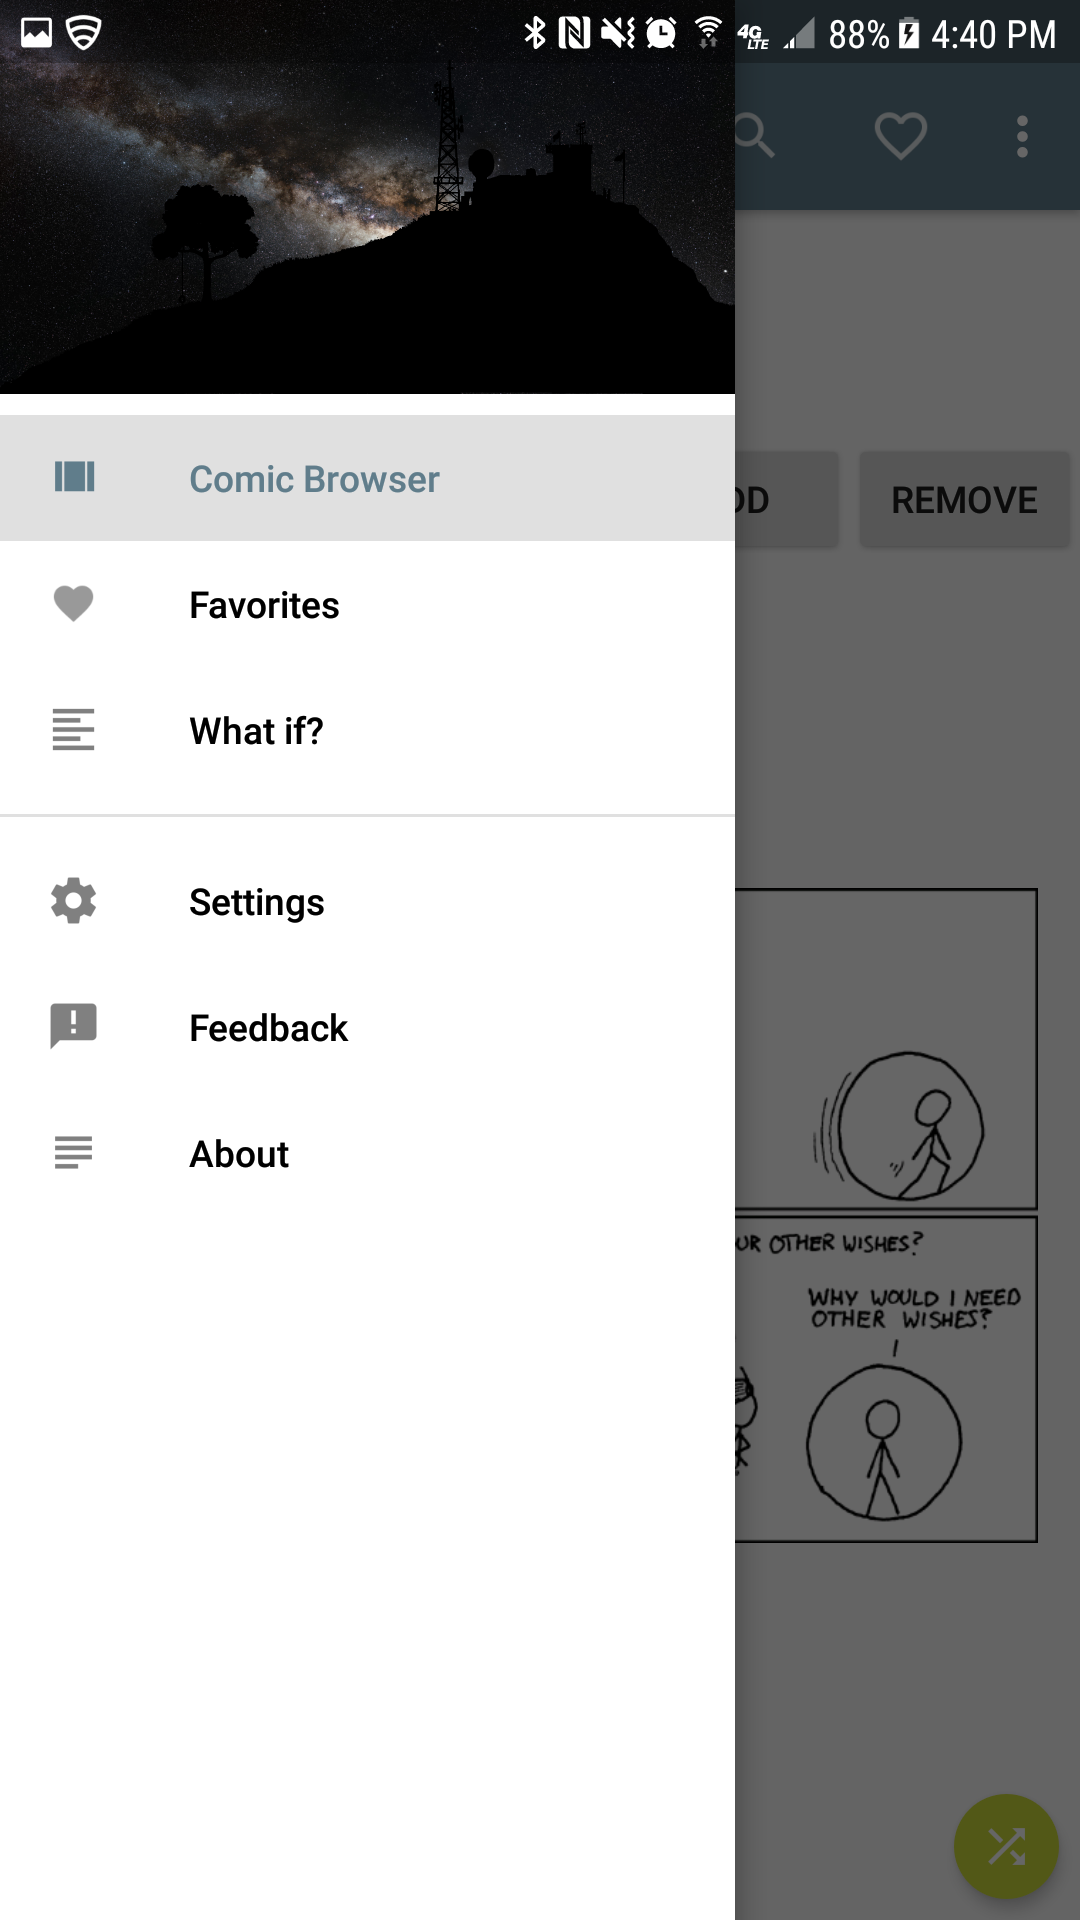
\includegraphics[width=\maxwidth{3in}]{img/t4s4.png}
		\centering
		\caption{Task 4 - Showing that the other functionality is the same}
	\end{figure}

\clearpage
\section{Task 5}
Deliverables: See Screenshots 17-20

Status Report: My application works. 
It's not especially fast, nor does it use many/very large word lists.
But if you use it you're pretty much guarnteed to have an extremely strong password because it's definition of a weak password is very strict. The application has only one activity for simplicity's sake.

Experience Report: This was probably my favorite application of the set.
I think it will be interesting to see how this plays out with rainbow tables and the cloud and such. As it is it's painfully slow right now.
Part of me wishes I had implemented progress reporting of some sort but I don't think it's worth it because the UI is "good enough" in my opinion, and I'm late enough as it is...

Definition of a similar password: My application defines a similar password as one which, after lowercasing the user password and the password in the dump, contains the dumped password, or which is a subset of the dump password. That is, I define it as follows, in code:

\begin{verbatim}
    if(dumpedPassword.toLowerCase().contains(userPassword))
        matches = true;

    if(userPassword.contains(dumpedPassword))
        matches = true;
\end{verbatim}

How helpful is this APK is: I believe this APK is the pretense of a future one, though I'm not really sure. It's pretty tightly bound to the UI unlike other solutions I have made in the past.
That said, I once looked at the docs about for the spark api, and it seems like streams are extremely easily ported from running locally to running on a cluster, so in that regard I think I will be well prepared for something like that.

    \begin{figure}[ht]
		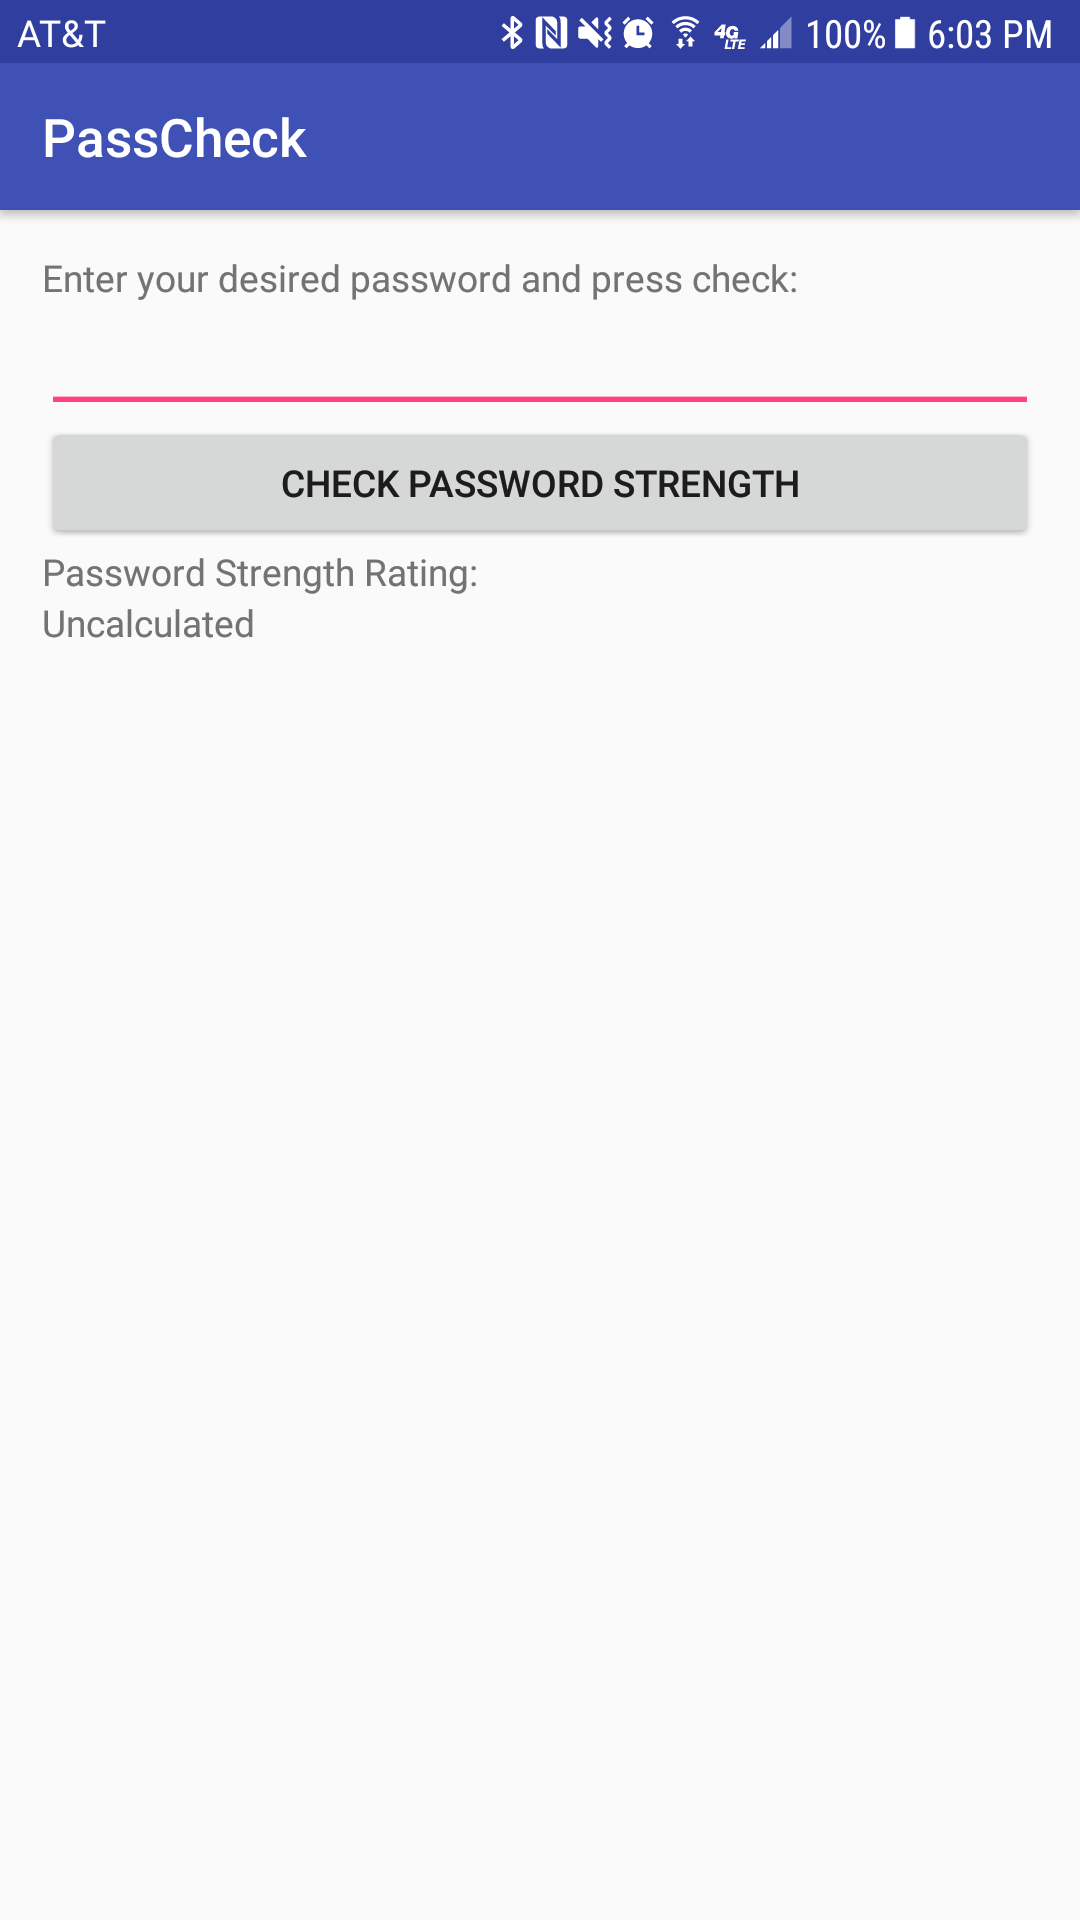
\includegraphics[width=\maxwidth{3in}]{img/t5s1.png}
		\centering
		\caption{Task 5 - The initial screen}
	\end{figure}
	\begin{figure}[ht]
		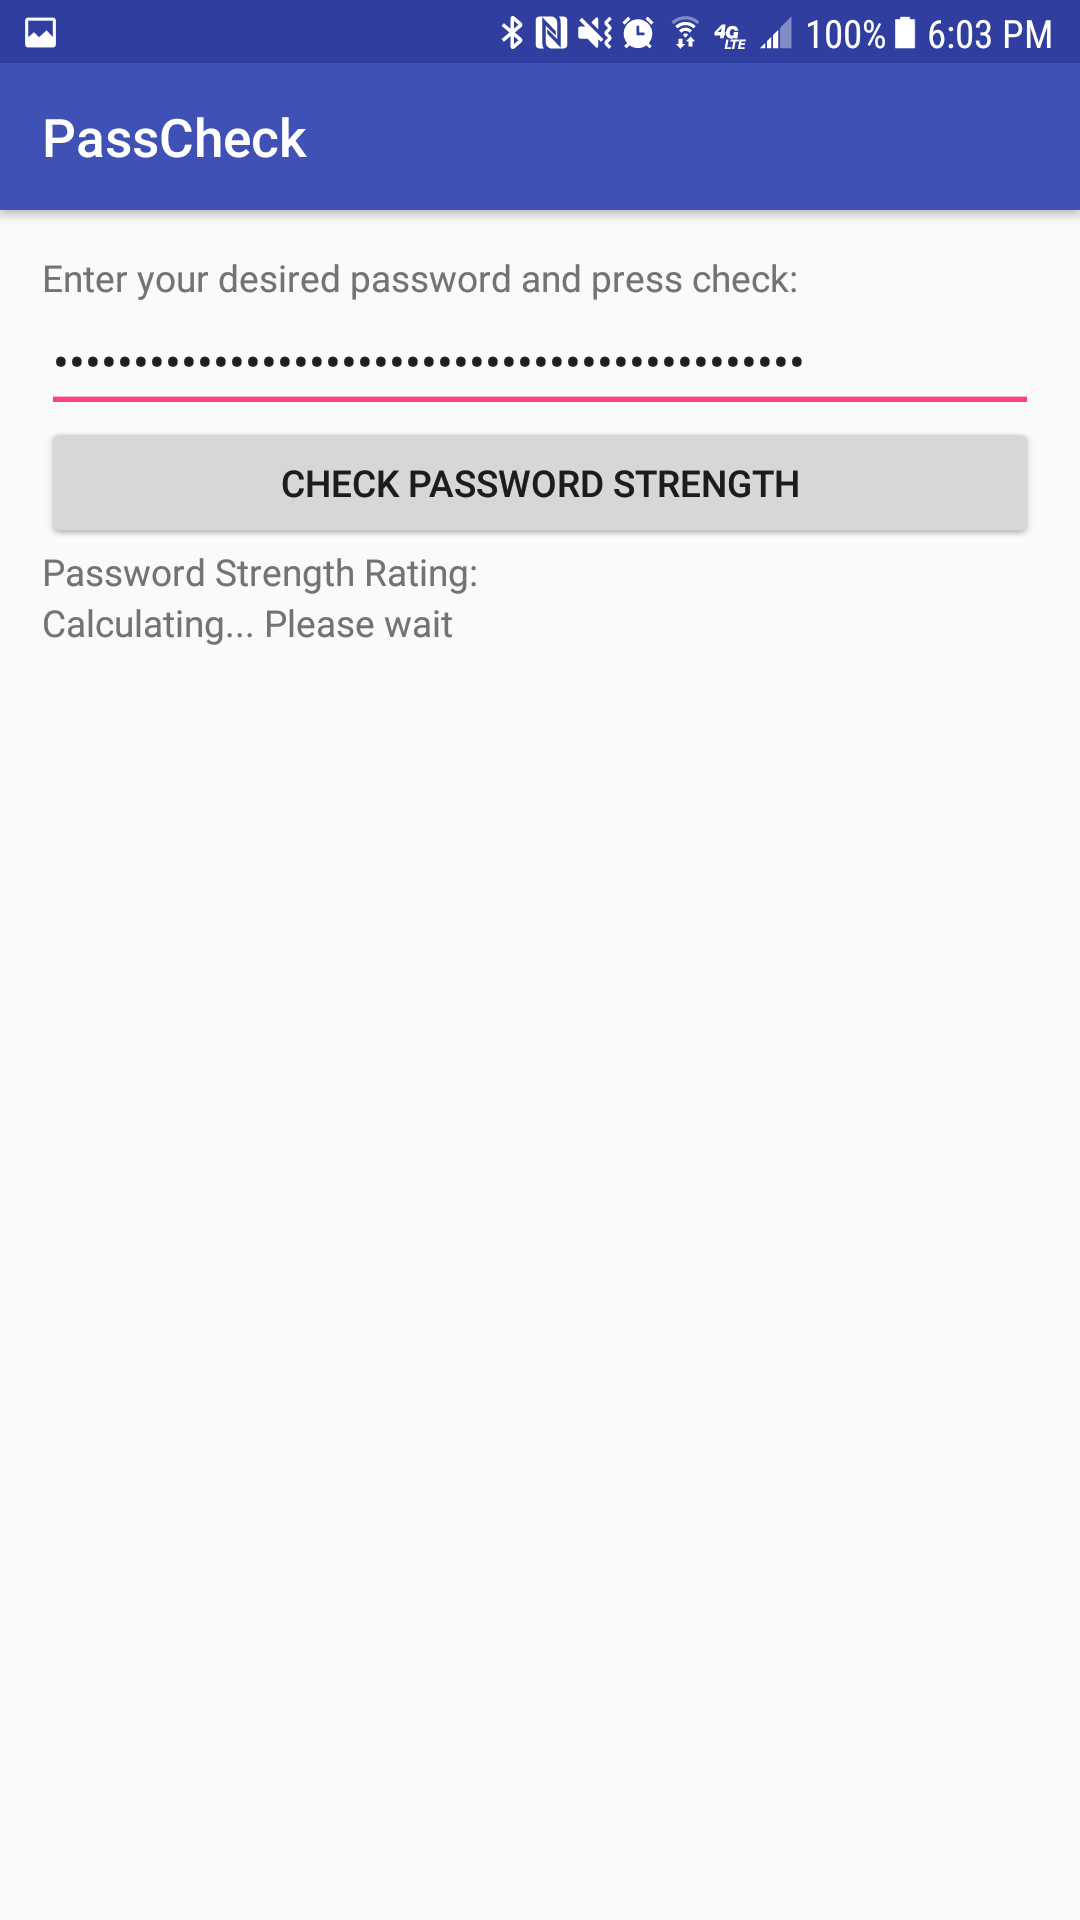
\includegraphics[width=\maxwidth{3in}]{img/t5s2.png}
		\centering
        \caption{Task 5 - Displayed to the user as it checks. Ideally I would put a progress report of some sort here, too.}
	\end{figure}
	\begin{figure}[ht]
		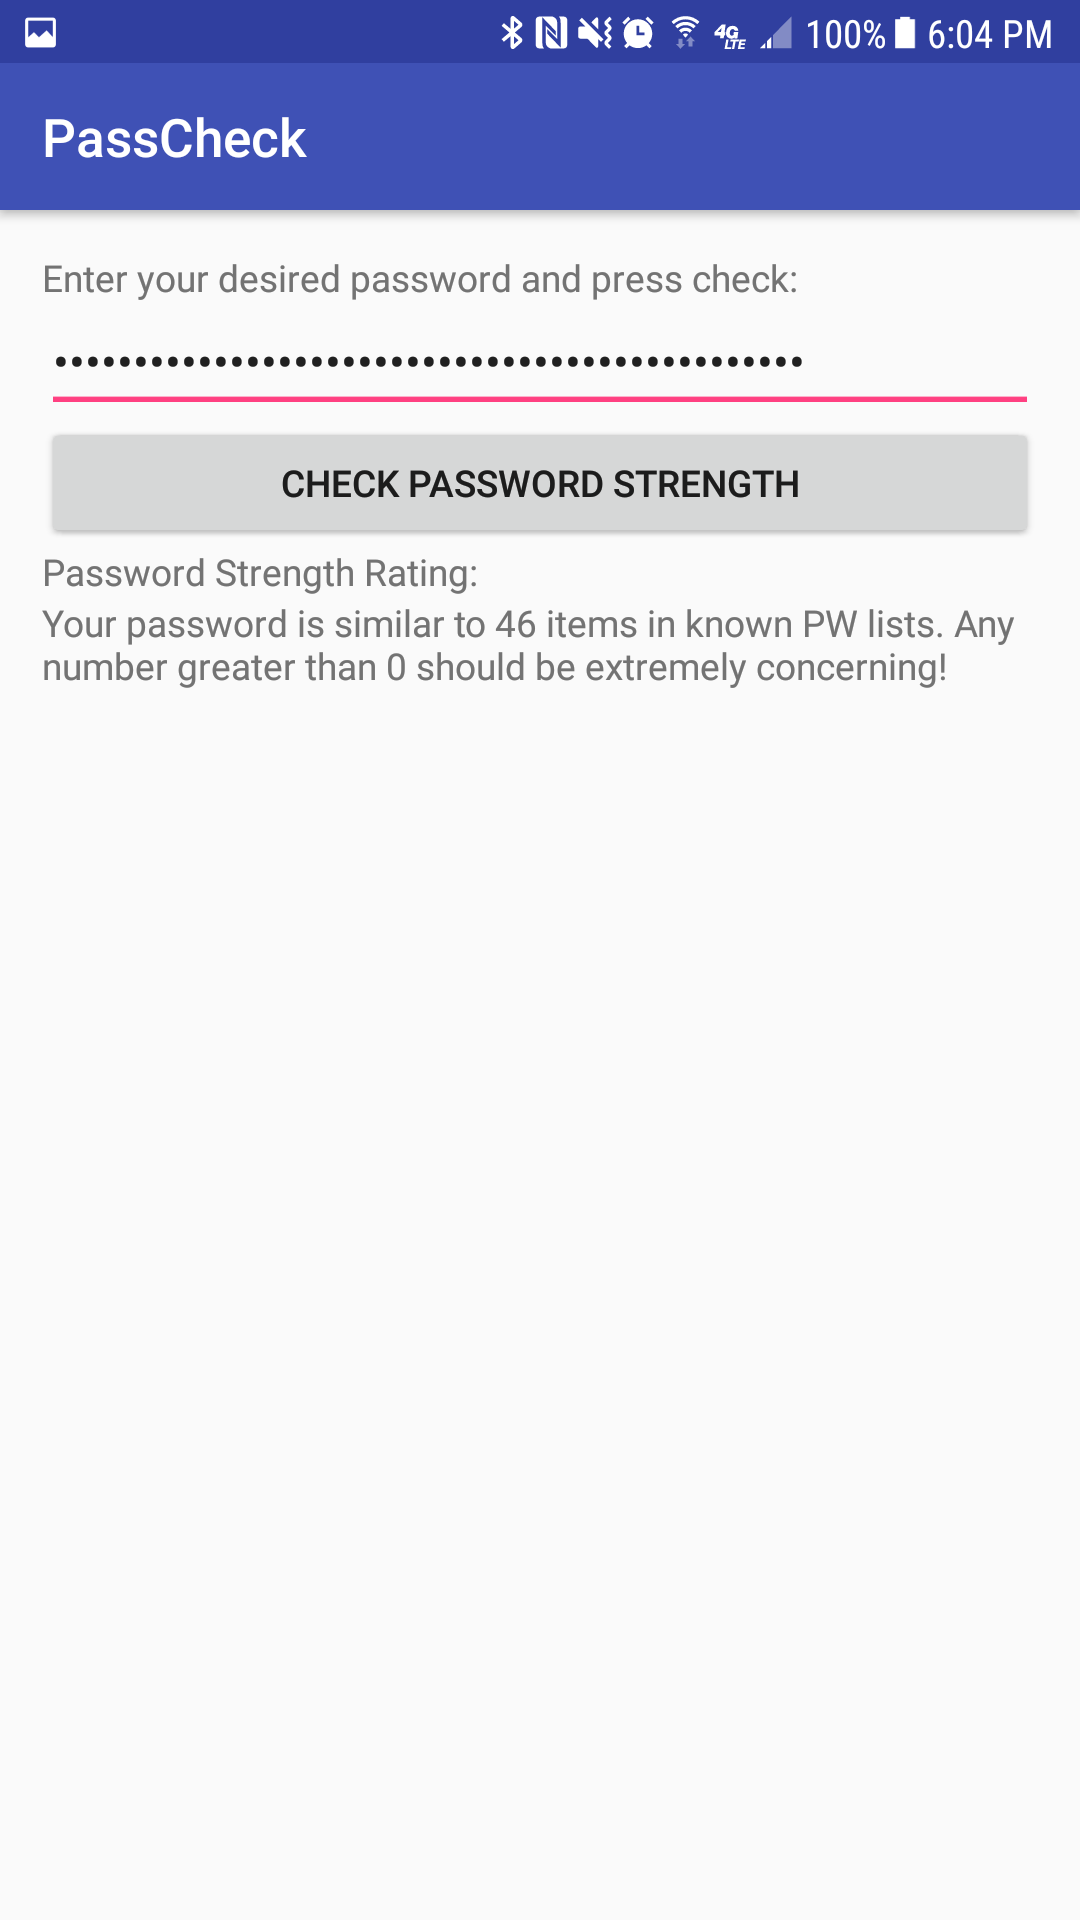
\includegraphics[width=\maxwidth{3in}]{img/t5s3.png}
		\centering
        \caption{Task 5 - Message displayed for passwords that are similar to ones in the wordlist}
	\end{figure}
	\begin{figure}[ht]
		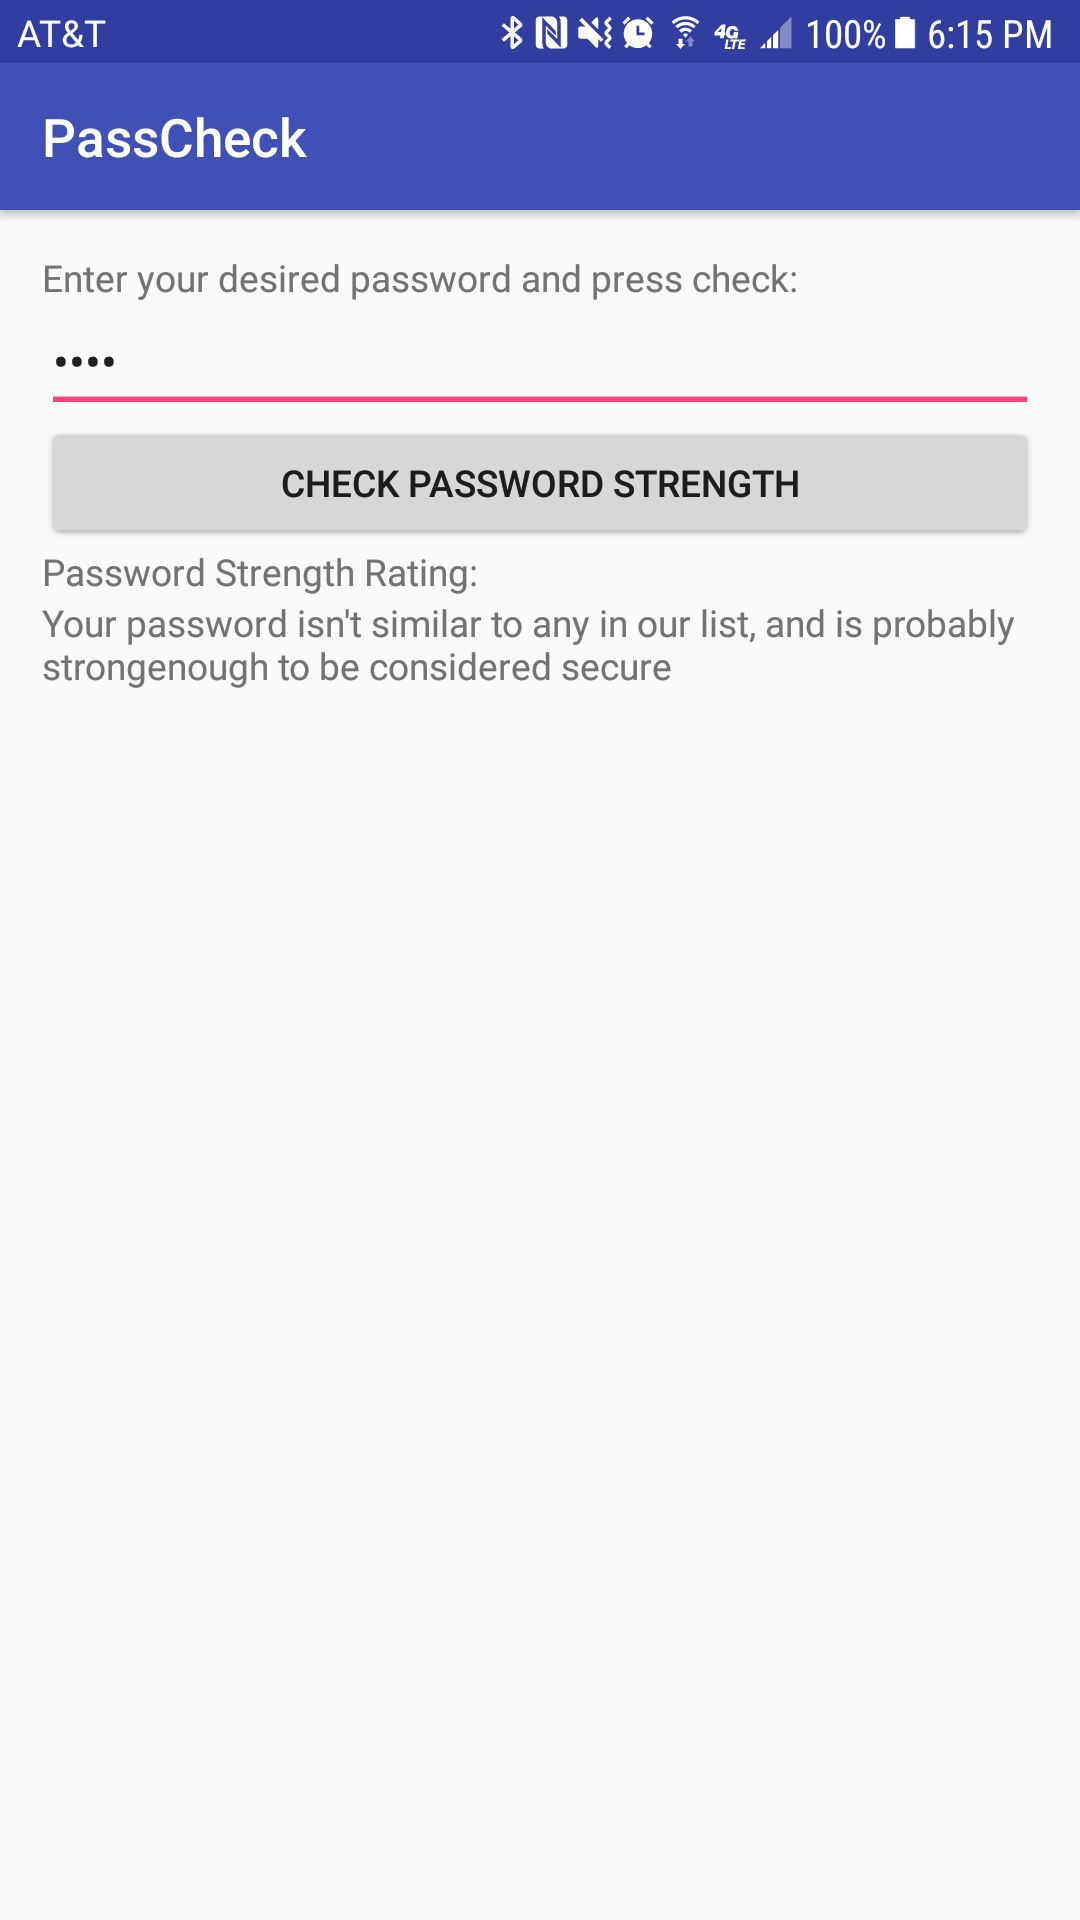
\includegraphics[width=\maxwidth{3in}]{img/t5s4.png}
		\centering
		\caption{Task 5 - Message displayed for passwords which are very strong}
    \end{figure}
\end{document}
